\documentclass[xcolor={svgnames},
  %hyperref={colorlinks,citecolor=Blue,linkcolor=Blue,urlcolor=DarkBlue}, 
  hyperref={colorlinks}, 
  spanish, 12pt]{beamer}
  \mode<presentation>
  
  \usefonttheme[onlymath]{serif}
  \setbeamertemplate{theorems}[ams style] 
  
  
\usetheme{metropolis}
 \useinnertheme{rectangles} 
\setbeamertemplate{navigation symbols}{}
%\setbeamertemplate{caption}[numbered]
%\useoutertheme{infolines}
\usepackage{cleveref}

\setbeamercovered{highly dynamic}

\newcounter{saveenumi}
\newcommand{\seti}{\setcounter{saveenumi}{\value{enumi}}}
\newcommand{\conti}{\setcounter{enumi}{\value{saveenumi}}}

\resetcounteronoverlays{saveenumi}

%\usepackage{beamerthemebars}
\usepackage{fontenc}
\usepackage{graphicx}
\usepackage[utf8]{inputenc}
\usepackage[spanish,mexico]{babel}
\usepackage{fontenc}
\usepackage{amsmath}
\usepackage{amsthm}
\usepackage{amssymb}
\usepackage{graphicx}
\usepackage{mathrsfs}
\usepackage{yfonts}
%\usepackage{hyperref}
\usepackage{enumerate}ntent/tweet
\usepackage{mathtools}
\usepackage{textcomp}
\usepackage{lmodern}
\usepackage{fancyvrb}
\usepackage{multicol}
\usepackage{color}
\usepackage{verbatim}

\DefineVerbatimEnvironment{ColorVerbatim}{Verbatim}%
  {formatcom=\color{purple},commandchars=\\\{\}}
  
\usepackage{etoolbox}

\BeforeBeginEnvironment{Verbatim}{\begingroup\color{purple}}%
\AfterEndEnvironment{Verbatim}{\endgroup}%
%\usepackage{etoolbox}
% \AtBeginEnvironment{enumerate}{\begin{multicols}{2}}    %%% this line
% \AtEndEnvironment{enumerate}{\end{multicols}}            %%% and this one
% \usepackage{multicol}
%\usepackage[usenames,dvipsnames,svgnames,table]{xcolor}
%\usepackage[urlcolor=blue]{hyperref}
%\numberwithin{section}{part}
\numberwithin{equation}{section} %% Comment out for sequentially-numbered
\numberwithin{figure}{section} %% Comment out for sequentially-numbered

% Automatically generate section title slides in beamer?
% Add support for \subsubsectionpage
\def\subsubsectionname{\translate{}}
\def\insertsubsubsectionnumber{\arabic{subsubsection}}
\setbeamertemplate{subsubsection page}
{
  \begin{centering}
    {\usebeamerfont{subsubsection name}\usebeamercolor[fg]{subsubsection name}\subsubsectionname}%~\insertsubsubsectionnumber}
    \vskip1em\par
    \begin{beamercolorbox}[sep=4pt,center]{part title}
      \usebeamerfont{subsubsection title}\insertsubsubsection\par
    \end{beamercolorbox}
  \end{centering}
}
\def\subsubsectionpage{\usebeamertemplate*{subsubsection page}}

\AtBeginSection{\frame{\sectionpage}}
\AtBeginSubsection{\frame{\subsectionpage}}
\AtBeginSubsubsection{\frame{\subsubsectionpage}}

\theoremstyle{plain}
  \newtheorem{thm}{Teorema}[section]
  \newtheorem{prop}{Proposici\'on}[section]
  \newtheorem{lem}[thm]{Lema}
  \newtheorem{cor}[thm]{Corolario}
  %\newtheorem{rem}{Observaci\'on}[chapter]
  \newtheorem*{sol}{Soluci\'on}
  \newtheorem{alg}{Algoritmo}[section]
  \newtheorem{solved}{Ejercicio Resuelto}
  \newtheorem{evc}{Evaluaci\'on Continua}

\theoremstyle{definition}
  \newtheorem{defn}{Definici\'on}[section]
  \newtheorem{conj}{Conjectura}[section]
  \newtheorem{exmp}{Ejemplo}[section]
  \newtheorem{exe}{Evaluaci\'on Continua}[section]
  \newtheorem{prob}{Problema}[section]
  \newtheorem{rem}{Observaci\'on}[section]
  \newtheorem*{ax}{Axioma}
  \newtheorem{tdv}{Tabla de Verdad}

\theoremstyle{remark}
  \newtheorem{claim}{Afirmaci\'on}[section]
  %\newtheorem{rem}{Observaci\'on}[chapter]
  %\newtheorem*{note}{Nota}
  \newtheorem{case}{Caso}
  \newtheorem{hint}{Sugerencia}[section]


\numberwithin{equation}{section}
\newcommand{\p}{\partial}
%\newcommand{\T}{\mathbb{T}}
\newcommand{\R}{\mathbb{R}}
\newcommand{\N}{\mathbb{N}}
\newcommand{\Q}{\mathbb{Q}}
\newcommand{\abs}[1]{\left|#1\right|}
\newcommand{\f}{\phi}
\newcommand{\vphi}{\varphi}
\newcommand{\vf}{\varphi}
\newcommand{\flow}[2]{\varphi^{#1}\left( #2 \right)}
\renewcommand{\d}[1]{\dot{#1}}
\renewcommand{\r}{\rho}
\newcommand{\A}{\mathcal{A}}
\newcommand{\gam}{\gamma}
\newcommand{\lam}{\lambda}
\renewcommand{\a}{\alpha}
\renewcommand{\b}{\beta}
\newcommand{\om}{\omega}
\newcommand{\iso}{\simeq}
\newcommand{\tensor}{\otimes}
\newcommand{\Z}{\mathbb{Z}}
\newcommand{\set}[1]{\left\{ #1 \right\}}
\newcommand{\inc}{\hookrightarrow}
\renewcommand{\L}{\mathcal{L}}
\renewcommand{\H}{\mathcal{H}}
\newcommand{\D}{\mathcal{D}}
\newcommand{\converge}[1]{\xrightarrow{#1}}
\renewcommand{\cot}{T^{*}}
\newcommand{\cott}[1]{T^{*}\T^{#1}}
\newcommand{\ep}{\epsilon}
\newcommand{\inp}[1]{\langle #1 \rangle}
%\newcommand{\G}{\mathcal{G}}
\newcommand{\hu}{\textbf{h}}
\newcommand{\deck}[1]{\operatorname{Dake}\left( #1 \right)}
\newcommand{\til}[1]{\tilde{#1}}
\newcommand{\Gam}{\Gamma}
\newcommand{\grad}{\nabla}
\newcommand{\del}{\delta}
\newcommand{\id}{\operatorname{Id}}
\newcommand{\Del}{\Delta}
\newcommand{\var}{\Delta}
\newcommand{\avch}[2]{\frac{\Delta #1}{\Delta #2}}
\newcommand{\Avch}[2]{\dfrac{\Delta #1}{\Delta #2}}
\newcommand{\Err}{\operatorname{Err}}
\newcommand{\imply}{\rightarrow}
\newcommand{\wed}{\wedge}
\newcommand{\biconditional}{\longleftrightarrow}
\newcommand{\yields}{\vdash}
\newcommand{\onlyif}{\Rightarrow}
\newcommand{\uset}{\mathbb{U}}
\newcommand{\minus}{\backslash}
\newcommand{\symdif}{\oplus}
\newcommand{\rel}[1]{\boxed{{\color{blue}\textbf{#1}}}}
\newcommand{\dom}[1]{\operatorname{Dom}\left( #1 \right)}
\newcommand{\im}[1]{\operatorname{Im}\left( #1 \right)}
\newcommand{\nrel}[1]{\boxed{{\color{red}\not}{\color{orange}\textbf{#1}}}}
\newcommand{\comp}[2]{#1 \circ #2}

%\date{\today}
\title{Matem\'aticas Discretas \\
Teor\'ia de Conjuntos}
\author[Juliho Castillo]{\href{https://www.youtube.com/channel/UCb1i-EtybaWWX5urFfmMUWQ}{M. en C. Juliho Castillo}}

\institute[ITESM-CCM]{Tec de Monterrey, Campus Ciudad de M\'exico}
\date{\today}

\begin{document}

\logo{
 
\includegraphics[width=3cm,keepaspectratio=true]{./logo.png}
 %LOGO-CECYTEO.png: 200x200 pixel, 72dpi, 7.06x7.06 cm, bb=0 0 200 200
}

\frame{
\titlepage
}

\begin{frame}[allowframebreaks=0.5]
 \tableofcontents
\end{frame}

%\frame{\tableofcontents}

% \AtBeginSubsection[]
% {
%   \begin{frame}
%     \tableofcontents[currentsubsection]
%   \end{frame}
% }
\section{Teor\'ia de Conjuntos}

\subsection{Conjuntos y Elementos. Subconjuntos}

\begin{frame}
 Un \emph{conjunto} puede ser visto como un conjunto bien definido de objetos, llamados \emph{elementos} o \emph{miembros} de tal conjunto. \pause
 
 Usualmente, usaremos letras may\'usculas para denotar conjunto, y min\'usculas para dlos elementos. 
\end{frame}

\begin{frame}
 La pertenencia en un conjunto se denota de la siguiente manera:
 \begin{center}
  \emph{$a \in S$ denota que $a$ pertenece al conjunto $S.$} \pause
  
  \emph{$a,b \in S$ denota que tanto $a$ como $b$ pertenecen al conjunto $S.$}
 \end{center}

 El s\'imbolo $\in$ significa \texttt{``es elemento de''.} \pause Por el contrario, $\notin$ significa \texttt{``no es elemento de''.}
\end{frame}

\subsubsection{Especificaci\'on de Conjuntos}

\begin{frame}
 B\'asicamente, existen dos maneras de especificar un conjunto en particular. \pause Por un lado, si es posible, enlistar todos los miembros. \pause Por otro lado, caracterizando los elementos en el conjunto.
\end{frame}

\begin{frame}
 En cualquier caso, para declarar un conjunto se utilizan llaves:
 $$
 A=\set{\cdots}
 $$
\end{frame}

\begin{frame}
 Por ejemplo, el conjunto 
 $$
 A=\set{1,3,5,6,9}
 $$
 tambi\'en se puede especificar como
 $$
 A=\set{x\in \N \mid x<10, 2\nmid x }
 $$
\end{frame}

\begin{frame}
 Un conjunto no depende del modo en que sus elementos se muestren. \pause Este permanece igual si sus elementos se repiten o se reacomodan.
\end{frame}


\begin{frame}
 \begin{exmp}
  \begin{align}
   \set{x\in\R | x^{2}-3x+2=0} & =\set{1,2} \\
   &=\set{1,2,2,1}
  \end{align}

 \end{exmp}

\end{frame}

\subsubsection{Subconjuntos}

\begin{frame}
 Supongamos que cada elemento en un conjunto $A$ es tambi\'en elemento del conjunto $B,$ es decir,
 $$
 x\in A \onlyif x\in B.
 $$
\end{frame}

\begin{frame}
 En ese caso, decimos que $A$ es subconjunto de $B.$ \pause Tambi\'en podemos decir que $A$ est\'a contenido en $B$ o que $B$ contiene a $A$.
\end{frame}

\begin{frame}
 Esta relaci\'on se escribe como
 $$
 A \subset B 
 $$ o en ocasiones como
 $B\supset A.$ \pause Por el contrario, si es necesario indicar que $A$ \emph{no} es  subconjunto de $B,$ escribimos $A \not\subset B.$
\end{frame}

\begin{frame}
 Diremos que dos conjuntos son iguales si poseen los mismos elementos, es decir, 
 $$
 x \in A \iff x \in B.
 $$
\end{frame}

\begin{frame}
 De manera equivalente 
 \begin{center}
  $A=B$ si y solo si $A \subset B$ y $B \subset A.$
 \end{center}

\end{frame}

\begin{frame}
 \begin{exmp}
  \label{lip:exmp:1.2}
  Determine la relaci\'on entre los siguientes conjuntos
  \begin{center}
   $$A=\set{1,3,4,7,8,9}, \, 
   B=\set{1,2,3,4,5}, \,
   C=\set{1,3}.$$
  \end{center}

 \end{exmp}

\end{frame}

\begin{frame}
 \begin{exmp}
  Demuestre que 
  \begin{enumerate}
   \item $A\not\subset B$ si y solo $\exists x\in A: x\notin B.$
   \item $A \subset A.$
   \item $A\subset B, B\subset C \onlyif  A\subset C.$
  \end{enumerate}

 \end{exmp}

\end{frame}

\subsubsection{S\'imbolos especiales}

\begin{frame} Algunos conjuntos num\'ericos tienen una notaci\'on especial
 \begin{itemize}
  \item $\N:$ n\'umeros naturales (enteros positivos); \pause
  \item $\Z:$ n\'umeros enteros; \pause
  \item $\Q:$ n\'umeros racionales; \pause
  \item $\R:$ n\'umeros reales; \pause
  \item $\mathbb{C}:$ n\'umeros complejos.
 \end{itemize}
\pause

\end{frame}

\begin{frame}
 Observe que
$$
\N \subset \Z \subset \Q \subset \R \subset \mathbb{C},
$$ pero en ning\'un caso los conjuntos son iguales. 
\end{frame}

\subsubsection{Conjunto Universal y Conjunto Vac\'io}

\begin{frame}
 Todos los conjuntos bajo investigaci\'on en una apliaci\'on de teor\'ia de conjuntos se supone que pertenecen a un conjunto fijo m\'as grande llamado \emph{conjunto universo} $\uset,$ al menos que se indique otro caso.
\end{frame}

\begin{frame}
 Dado un conjunto universal $\uset$ y una propiedad $P,$ es posible que no existan elemento de $\uset$ con la propiedad $P.$ 
\end{frame}

\begin{frame}
 Por ejemplo, el siguiente conjunto no tiene elementos
 $$
 S=\set{x\in \Z \mid x^{2}=3}.
 $$
\end{frame}

\begin{frame}
 A tal conjunto sin elementos $\set{}$ se le conoce como conjunto vac\'io y se denota como $\emptyset.$
\end{frame}

\begin{frame}
 \begin{rem}
  \emph{S\'olo existe un conjunto vac\'io}. \pause El conjunto vac\'io es subconjunto de cualquier otro conjunto.
 \end{rem}

\end{frame}

\subsubsection{Conjuntos disjuntos}

\begin{frame}
Dos conjuntos $A$ y $B$ son \emph{disjuntos} si no tienen elementos en com\'un. 
\end{frame}

\begin{frame}
 \begin{exmp}
  Considere $$
  A=\set{1,2}, \; B=\set{4,5,6}, \; C=\set{5,6,7,8}.
  $$
  Determine que pares de conjuntos son disjuntos. 
 \end{exmp}

\end{frame}

\subsection{Diagramas de Venn}

\begin{frame}
 Un diagrama de Venn es una representaci\'on gr\'afica de conjuntos en el que cada conjunto est\'a representado por \'areas encerradas en el plano.
\end{frame}

\begin{frame}
 El conjunto universo $\uset$ es representado por el interior de un rect\'angulo, y cualquier otro conjunto esta representado por discos que viven dentro del rect\'angulo.
\end{frame}

\begin{frame}
 \begin{figure}
 \centering
 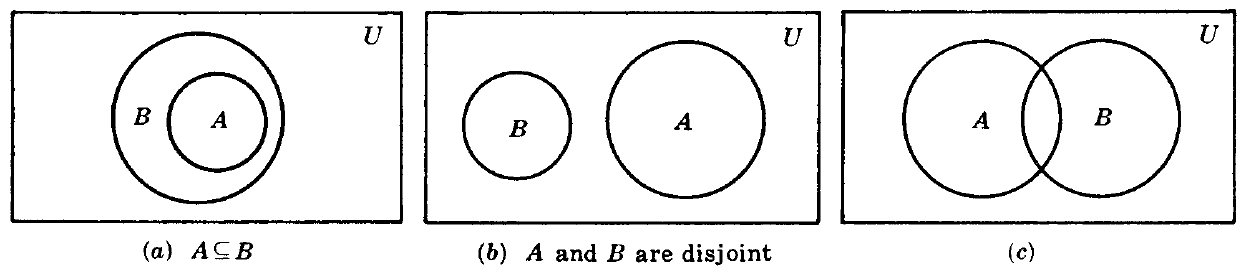
\includegraphics[width=11cm,keepaspectratio=true]{./venn01.png}
 % venn01.png: 0x0 pixel, 300dpi, 0.00x0.00 cm, bb=
 \caption{Representaciones con Diagramas de Venn}
 \label{fig:0101}
\end{figure}

\end{frame}

\subsection{Operaciones con Conjuntos}

\begin{frame}
 En esta secci\'on introduciremos la uni\'on, la intersecci\'on y el complemento de conjuntos.
\end{frame}

\subsubsection{Uni\'on e Intersecci\'on}

\begin{frame}
 La uni\'on de dos conjuntos $A$ y $B$ es el conjunto de todos los elementos que pertenecen a $A$ o a $B,$ \pause es decir
 $$
 A \cup B = \set{x \mid x\in A \vee x\in B}.
 $$
\end{frame}

\begin{frame}
 La intersecci\'on de dos conjuntos $A$ y $B$ es el conjunto de todos los elementos que pertenecen a $A$ y a $B,$ \pause es decir
 $$
 A \cap B = \set{x \mid x\in A \wed x\in B}.
 $$
\end{frame}

\begin{frame}
 \begin{figure}
 \centering
 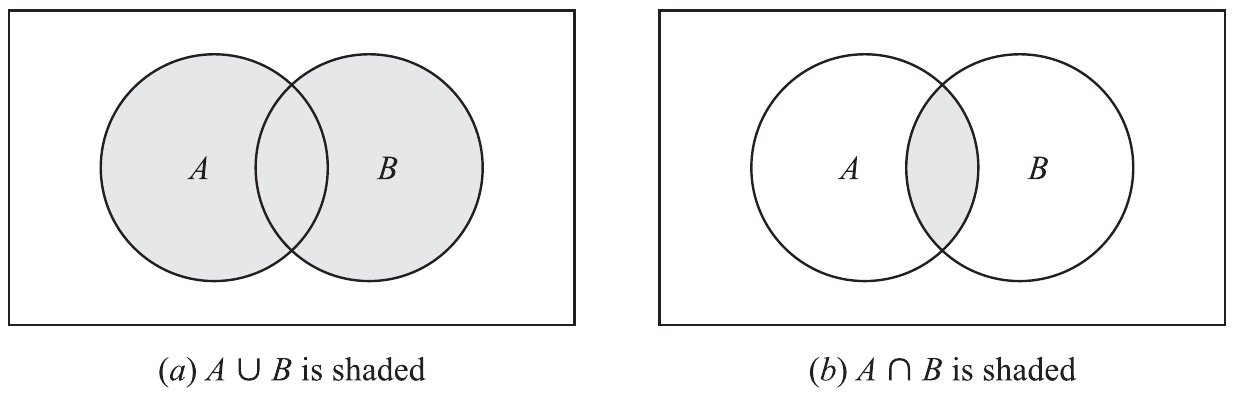
\includegraphics[width=10cm,keepaspectratio=true]{./venn_union_interseccion.png}
 % venn_union_interseccion.png: 0x0 pixel, 300dpi, 0.00x0.00 cm, bb=
 \caption{Unión e Intersección}
 \label{fig:0103}
\end{figure}

\end{frame}


\begin{frame}
 \begin{exmp}
  \label{lip:exmp:1.4.a}
  Sea $A=\set{1,2,3,4},$ $B=\set{3,4,5,6,7},$ $C=\set{2,3,8,9}.$ Encuentre 
  \begin{enumerate}
   \item $A \cup B=$ \pause
   \item $A \cap B=$ \pause
   \item $A \cup C=$ \pause
   \item $A \cap C=$ \pause
   \item $B \cup C=$ \pause
   \item $B \cap C=$
  \end{enumerate}

 \end{exmp}

\end{frame}

\begin{frame}
 \begin{exmp}
  \label{thm:1.3}
  Demuestre que para cualesquiera dos conjuntos $A$ y $B,$ tenemos:
  $$
  A \cap B \subset A \subset A \cup B.
  $$
 \end{exmp}

\end{frame}

\begin{frame}
 \begin{exmp}
  \label{thm:1.4}
  Demuestre que las siguientes proposiciones son equivalentes:
  \begin{enumerate}
   \item $\displaystyle A \subset B$
   \item $\displaystyle A \cap B = A$
   \item $\displaystyle A \cup B = B$
  \end{enumerate}

 \end{exmp}

\end{frame}

\begin{frame}
 Dos conjuntos $A$ y $B$ se dicen \emph{disjuntos} si no tienen elementos en com\'un, es decir $A\cap B=\emptyset$.
 \pause
 
 Supongamos que 
 $$
 S=A\cup B, \; A\cap B=\emptyset.
 $$ \pause Diremos que $S$ es la uni\'on disjunta de $A$ y $B$ y se denota por $$S=A \sqcup B.$$ 
 
\end{frame}

\subsubsection{Complementos, Diferencias y Diferencias Sim\'etricas}

\begin{frame}
 En esta secci\'on, consideraremos conjuntos que sean subconjuntos de un conjunto universo fijo $\uset.$
\end{frame}

\begin{frame}
 El \emph{complemento} $A^{C}$ de un conjunto $A$ es el conjunto de elementos que no pertenecen a $A$, es decir 
 $$A^{C}=\set{x\in \uset \mid x \notin A}.$$
\end{frame}

\begin{frame}
 Algunos textos denotan $A^{C}$ tambi\'en como $A'$ o $\bar{A}.$ 
\end{frame}

\begin{frame}
 El \emph{complemento relativo} de un conjunto $B$ con respecto a un conjunto $A$ se define como 
 $$
 A\minus B = \set{x \mid x \in A, x \notin B}.
 $$
\end{frame}

% \begin{frame}
%  \begin{exmp}
%   Demuestre que 
%   $A \minus B = A \cap B^{C}$
%  \end{exmp}
% 
% \end{frame}


\begin{frame}
 El conjunto $A\minus B$ se lee \texttt{$A$ menos $B$.} Algunos textos lo denotan tambi\'en como $A-B.$  
\end{frame}

\begin{frame}
 La \emph{diferencia sim\'etrica} de los conjuntos $A$ y $B$ se define como $$A\symdif B=\left( A\cup B \right)\minus \left( A \cap B \right).$$
\end{frame}

\begin{frame}
 \begin{figure}
 \centering
 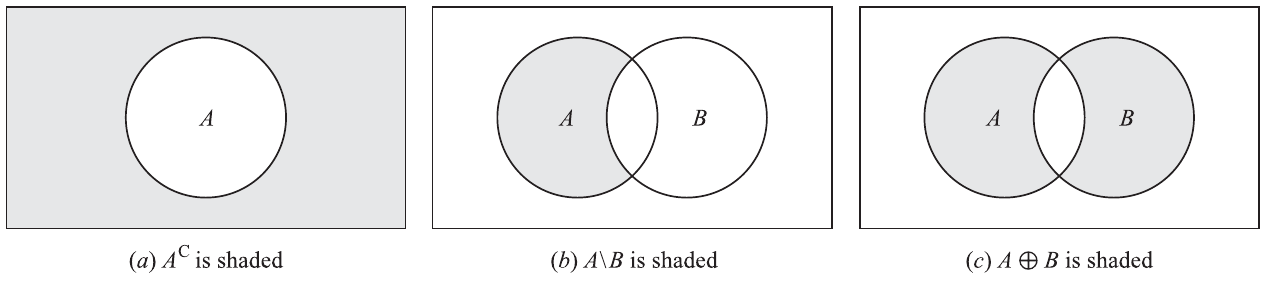
\includegraphics[width=10cm,keepaspectratio=true]{./venn_complemento.png}
 % venn_complemento.png: 0x0 pixel, 300dpi, 0.00x0.00 cm, bb=
 \caption{Complementos, diferencia y diferencia simétrica.}
 \label{fig:0104}
\end{figure}

\end{frame}

\begin{comment}
\begin{frame}
 \begin{exmp}
  Definamos $$p\veebar q \equiv \left( p \vee q \right) \wed \neg\left( p \wed q \right)$$
 Demuestre que 
 \begin{enumerate}
  \item $ \displaystyle
   x \in A\symdif B \iff \left( x \in A \right) \veebar \left( x \in B  \right)
   $ \pause
   \item $\displaystyle p\veebar q \equiv \left( p \wed \neg q \right) \vee \left( q \wed \neg p \right)$ \pause
   \item $\displaystyle A \veebar B = \left( A \minus B \right) \cup \left( B \minus A \right)$
 \end{enumerate}

 \end{exmp}

\end{frame}

\begin{frame}
 \begin{exmp}
  \label{lip:exmp:1.5}
  Supongamos que $\N$ es el conjunto universo. Definamos $A=\set{1,2,3,4},$ $B=\set{3,4,5,6,7},$ $C=\set{2,3,8,9},$ $E=\set{2,4,6,...}.$
 
 Determine:
 \begin{enumerate}
  \item $A \symdif B$ \pause
  \item $A \symdif C$ \pause
  \item $B \symdif C$ \pause
  \item $A \symdif E$
 \end{enumerate}
\end{exmp}
\end{frame}


\subsubsection{Conjuntos fundamentales}

\begin{frame}
 Dos conjuntos $A$ y $B$ se dicen \emph{disjuntos} si no tienen elementos en com\'un, es decir $A\cap B=\emptyset$.
 \pause
 
 Supongamos que 
 $$
 S=A\cup B, \; A\cap B=\emptyset.
 $$ \pause Diremos que $S$ es la uni\'on disjunta de $A$ y $B$ y se denota por $$S=A \sqcup B.$$ 
 
\end{frame}

\begin{frame}
 En general $S$ es una uni\'on disjunta de $P_{1}, P_{2},...,P_{n}$ si 
 \begin{itemize}
  \item $\displaystyle S=P_{1}\cup P_{2}\cup...\cup P_{n}$ y
  \item $P_{i}\cap P_{j}=\emptyset$ siempre y cuando $i\neq j.$
 \end{itemize}
\pause

En este caso, escribimos
$$
S=P_{1}\sqcup P_{2}\sqcup...\sqcup P_{n}.
$$
\end{frame}

\begin{frame}
 Diremos que $P_{1}, P_{2},...,P_{n}$ es sistema de conjuntos fundamentales para $\uset$ si
 $$
 \uset = P_{1}\sqcup P_{2}\sqcup...\sqcup P_{n}.
 $$
\end{frame}

\begin{frame}
 \begin{exmp}
  \label{lip:exmo:1.6}
  Contruya un sistema de conjuntos fundamentales a partir de tres conjunto $A, B, C.$  
  \end{exmp}
\end{frame}

\begin{frame}
 \begin{figure}
 \centering
 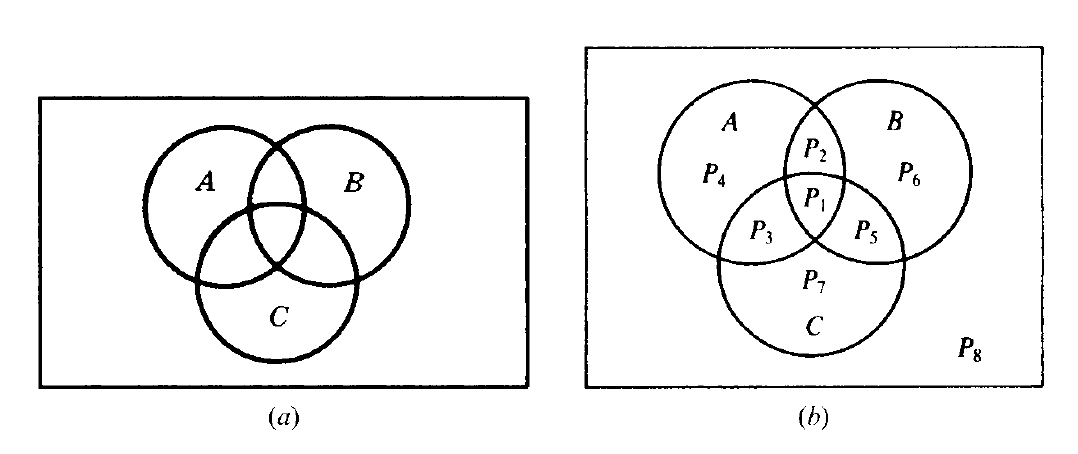
\includegraphics[width=10cm,keepaspectratio=true]{./sistema_fundamental.png}
 % sistema_fundamental.png: 0x0 pixel, 300dpi, 0.00x0.00 cm, bb=
 \label{fig:0105}
\end{figure}

\end{frame}
\end{comment}

\subsubsection{Álgebra de conjuntos, dualidad}

\begin{frame}
	Los conjuntos bajo las operaciones de unión, intersección y complemento satisface varias leyes o identidad, que se enuncian en la siguiente tabla, y son similares a las leyes de lógica.
\end{frame}

\begin{frame}
\begin{figure}
	\centering
	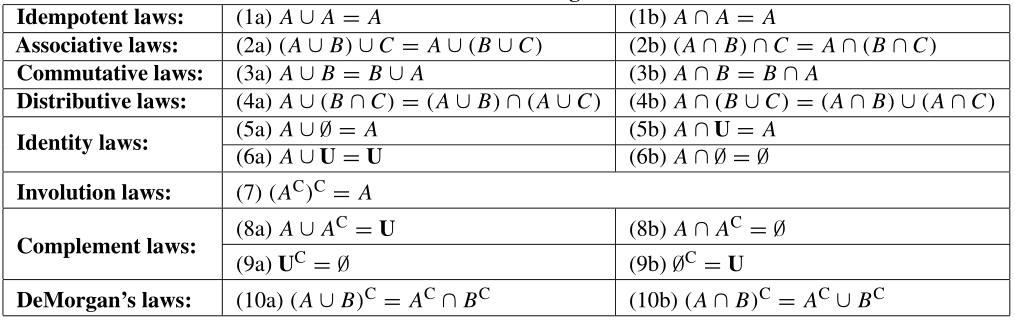
\includegraphics[width=11cm,keepaspectratio=true]{./leyes_conjuntos.png}
	\caption{Leyes de Conjuntos}
	\label{fig:leyesconjuntos}
\end{figure}

\end{frame}

\begin{frame}
	Cada ley de conjuntos se corresponde con una ley de lógica. Por ejemplo, la ley de DeMorgan:
	\begin{align*}
	\left(A \cup B\right)^{C} &= \set{x \mid x\notin(A \cup B)}\\
	&= \set{x \mid x\notin A \wed x\notin B}\\
	&=A^{C}\cap B^{C}
	\end{align*}
\end{frame}

\begin{frame}
	\frametitle{Dualidad}
	El \emph{principio de dualidad} establece que la equivalencia $E^{*}$ obtenida a partir de una ley de lógica $E$ reemplazando
	\[ \cup, \cap, \uset, \emptyset\] por
	\[ \cap, \cup, \emptyset, \uset\]
	sigue siendo una ley de lógica.
	\pause
	
	A la proposición $E^{*}$ se le conoce como dual $E.$
\end{frame}

\begin{frame}
	\begin{exmp}
		Encuentre el dual de 
		\[ (\uset \cap A) \cup (B\cap A) = A\]
	\end{exmp}
\end{frame}

\subsection{Inducci\'on Matem\'atica}

\begin{frame}
 Una propiedad esencial de los naturales $\N=\set{1,2,3,...}$  es la siguiente
 \pause
 
 \begin{ax}[Principio de Inducci\'on Matem\'atica, versi\'on I]
 Sea $P$ una proposici\'on definida en $\N,$ es decir, $P(n)$ toma valores de cierto o falso para cada $n\in \N.$
 
 Supongamos que
 \begin{enumerate}
  \item $P(1)$ es cierto;
  \item $\forall k \in \N: P(k) \onlyif P(k+1).$
 \end{enumerate}

 Entonces $P$ es cierto para todo entero positivo $n\in \N.$
 \end{ax}

\end{frame}

\begin{frame}[t]
\begin{exmp}
 Sea $P(n):1+3+5+...+(2n-1)=n^2.$ Demostrar que $P(n)$ es cierta para toda $n \in \N.$ 
\end{exmp}
\end{frame}

\begin{frame}
 \begin{ax}[Principio de Inducci\'on Matem\'atica, versi\'on II]
  Sea $P$ una proposici\'on definida en $\N$ tal que :
  \begin{enumerate}
   \item $P(1)$ es cierta;
   \item $P(k)$ es cierta siempre que $P(j)$ para toda $1\leq j < k.$
  \end{enumerate}
Entonces $P(n)$ es cierta para toda $n\in \N.$
 \end{ax}

\end{frame}

\begin{frame}
 \begin{rem}
  Algunas veces, uno desea demostrar que una proposici\'on es cierta para alg\'un conjunto de enteros
 $$
 \set{a,a+1, a+2,...}
 $$
 donde $a$ es un entero positivo, posiblemente cero. Esto puede hacerse simplemente reemplazando $1$ por $a$ en cualquier versi\'on del Principio de Inducci\'on Matem\'atica. 
 \end{rem}

\end{frame}

\begin{frame}[t]
 \begin{solved}
  Demostrar que $$P(n): 1+2+3+...+n=\frac{1}{2}n\left( n+1 \right)$$
  es cierto para todo $n \in \N.$
 \end{solved}

\end{frame}

\begin{frame}[t]
 \begin{solved}
  Demostrar que $$P(n): 1+2+2^{2}+...+2^{n}=2^{n+1}-1$$
  es cierto para todo $n \in \N.$
 \end{solved}

\end{frame}

\end{document}
